\documentclass{beamer}
\usecolortheme{beaver}

\usepackage[utf8]{inputenc}
\usepackage[spanish]{babel}
\usepackage{graphicx}
\usebackgroundtemplate%
{%
    
\includegraphics[width=\paperwidth]{Images/fondoguatejug}%
}

\title{Creando aplicaciones Web con JavaEE 7 y JBoss Forge}
\author{Víctor Orozco}
\institute{Nabenik}
\date{\today}

\begin{document}

\frame{\titlepage}

\section{Intro}

\section{JS}

\begin{frame}{JavaEE 7}
	\begin{figure}
		\centering
		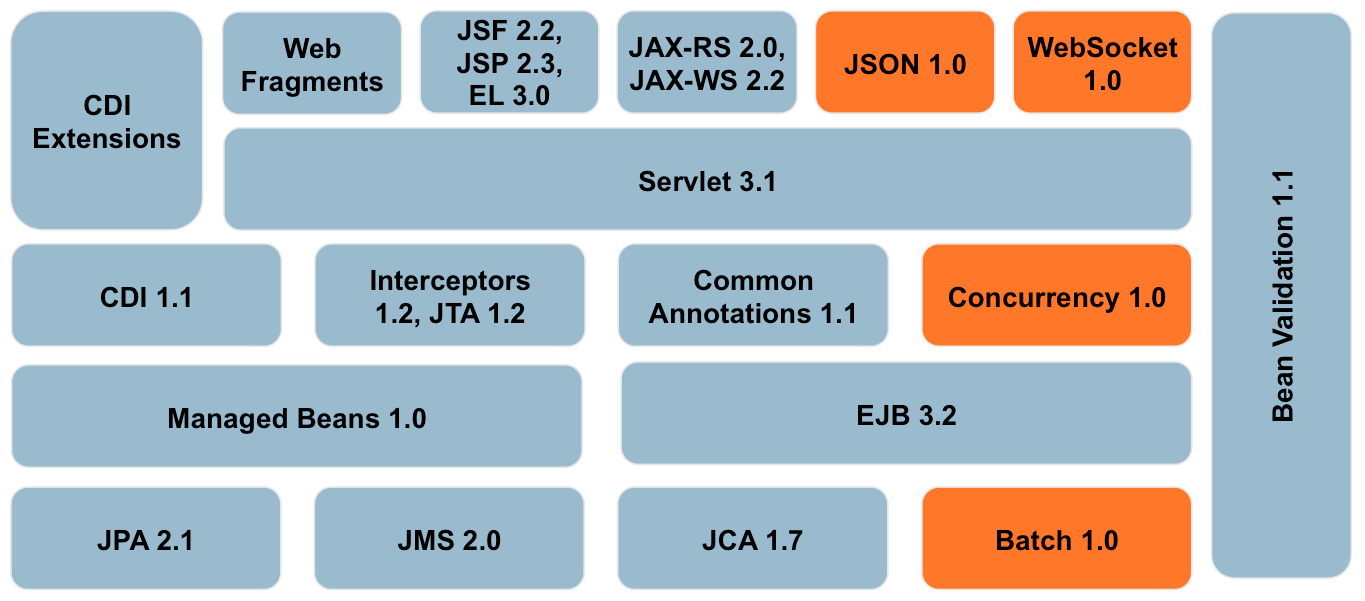
\includegraphics[width=0.9\linewidth]{Images/javaee7-pancake.png}
	\end{figure}	
\end{frame}

\begin{frame}{JavaEE 7}
	\begin{itemize}
		\item API Rest - JAX-RS 2.0
		\item WebSocket - WebSocket 1.0, Servlet 3.1
		\item JSON - JSON API 1.0
		\item SOA, Microservices
	\end{itemize}
	\begin{figure}
		\centering
		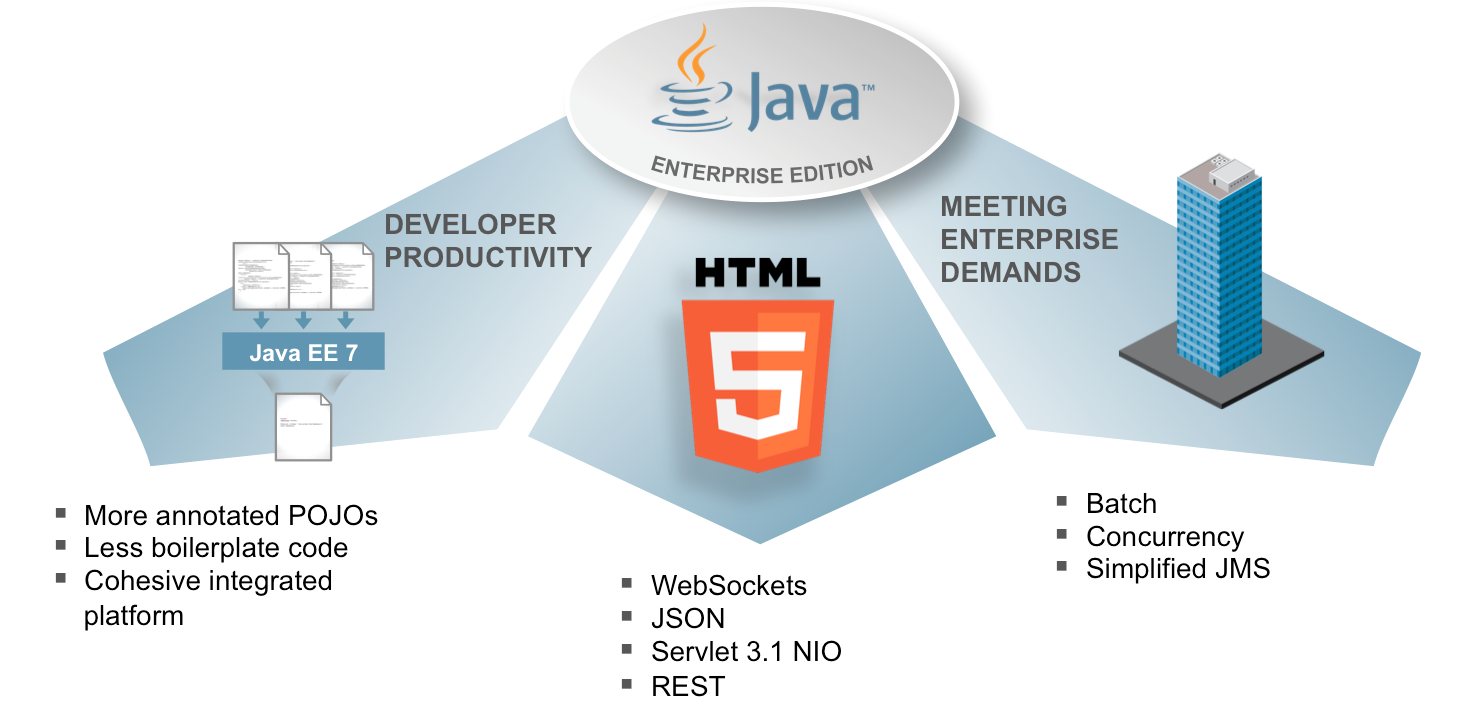
\includegraphics[width=0.7\linewidth]{Images/javaee7-theme}
	\end{figure}
\end{frame}

\begin{frame}{Arquitectura 2015}
	\begin{figure}
\centering
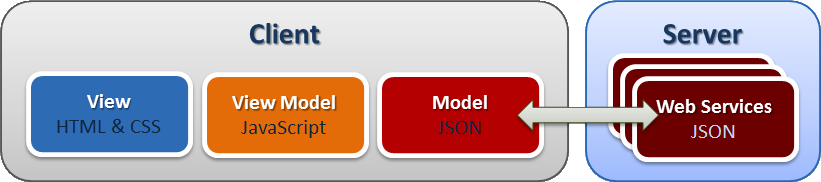
\includegraphics[width=0.9\linewidth]{Images/arq2015b}
\end{figure}
\end{frame}

\begin{frame}{JavaEE 7 - 2016}
	\begin{figure}
		\centering
		
\includegraphics[width=0.8\linewidth]{Images/anguaree.png}
	\end{figure}
\end{frame}


\begin{frame}{Ventajas}
	\begin{itemize}
		\item Existen n cantidad de bibliotecas JavaScript
		\item Independencia de backend
		\item Escalabilidad (stateless)
		\item Thin server apps
		\item Mejor tiempo de respuesta en comparación a JSF/SpringMVC
	\end{itemize}
\end{frame}

\begin{frame}{Desventajas}
	\begin{itemize}
		\item Existen n cantidad de bibliotecas JavaScript
		\item Complejidad y restricciones de REST
		\item AngularJS no sera compatible hacia atrás
	\end{itemize}
\end{frame}

\begin{frame}{Demo}
	\begin{itemize}
		\item Call for papers
		\item H2 + WildFly
		\item Bean Validation, JPA, JAX-RS, JSON
		\item AngularJS vanilla
		\item Forge
		\item http://github.com/tuxtor/cfp-angularjs-demo
	\end{itemize}
\end{frame}

\begin{frame}{QA}
	\begin{itemize}
		\item AngularJS - https://angularjs.org/
		\item JavaEE - http://docs.oracle.com/javaee/7/index.html
		\item Libros recomendados:
		\begin{itemize}
			\item Java EE 7 Essentials - Arun Gupta
			\item Developing RESTful Services with JAX-RS 2.0 - Masoud Kalali, Bhakti Mehta
			\item Eloquent JavaScript - Marijn Haverbeke
		\end{itemize}
	\end{itemize}
\end{frame}



\section{Fin}

\begin{frame}{Gracias}
\begin{itemize}
\item tuxtor@shekalug.org
\item http://tuxtor.shekalug.org
\item http://github.com/tuxtor/slides
\end{itemize}
\begin{center}

\includegraphics[width=0.1\linewidth]{Images/cclogo}
\\
This work is licensed under a Creative Commons Attribution-ShareAlike 3.0 Guatemala License.
\end{center}
\end{frame}
\end{document}
